\documentclass[main.tex]{subfiles}


\begin{document}

\section{Conservation in Systems}

\subsection{Momentum}

Momentum is a vector and has the same direction as velocity $v$. Since mass is a scalar, when velocity is in a negative direction (i.e., opposite the direction of motion), the momentum will also be in a negative direction; and when velocity is in a positive direction, momentum will be in a positive direction. The SI unit for momentum is \SI{}{kg\,m/s}.
\vspace{1em}

We may define \gls{change in momentum} ($\Delta p$) as the difference between final and initial values of momentum: $\Delta p = p_f - p_i$. Since the mass of an object rarely changes during short time intervals, change in momentum is associated with change in velocity:

\begin{equation} \label{dq0Ujw}
    \Delta p = m\,\Delta v = m \left(v_f - v_i\right)
\end{equation}

\begin{center}
    \begin{tabular}{cl|cl}
    \hline
    \textbf{Symbol} & \textbf{Quantity} & \textbf{SI Unit} & \textbf{Unit Symbol}  \\
    \hline\hline
    \rule{0pt}{2.5ex}
        $\Delta p$ & change in momentum & kilogram meter per second & \SI{}{kg\,m/s}\\
        $m$ & mass & kilogram & kg\\
        $\Delta v$ & change in velocity & meter per second & m/s\\
    \hline
        $v_f$ & final velocity & meter per second & m/s\\
        $v_i$ & initial velocity & meter per second & m/s\\
    \hline
    \end{tabular}
\end{center}

\begin{example} \label{EvkSMv}
    A 0.057-kg tennis ball moves at $-\SI{12}{m/s}$ when it gets struck to a new velocity of $+\SI{48}{m/s}$. What is the ball's change in momentum?
\end{example}

\begin{center}
\begin{tikzpicture}
\begin{axis}[
    width=8cm,height=3cm,
    axis line style={draw=none},
    ticks=none,
    axis lines=left,
    xmin=0,xmax=10,
    ymin=0,ymax=10,
    clip=false
]
    \fill[black!10] (5.4,5) circle (2mm);
    \fill[black!20] (5.2,5) circle (2mm) node[black,above=8pt] {$-\SI{12}{m/s}$};
    \fill (5,5) circle (2mm);
\end{axis}
\end{tikzpicture}%

\begin{tikzpicture}
\begin{axis}[
    width=8cm,height=3cm,
    axis line style={draw=none},
    ticks=none,
    axis lines=left,
    xmin=0,xmax=10,
    ymin=0,ymax=10,
    clip=false
]
    \fill[black!10] (5,5) circle (2mm);
    \fill[black!20] (5.4,5) circle (2mm) node[black,above=8pt] {$+\SI{48}{m/s}$};
    \fill (5.8,5) circle (2mm);
\end{axis}
\end{tikzpicture}%
\end{center}

\Solution We know the tennis ball's mass, initial velocity, and final velocity: $m = \SI{0.057}{kg}$, $v_i = -\SI{12}{m/s}$, and $v_f = +\SI{48}{m/s}$. We want to find change in momentum: $\Delta p =\ ?$ Change in momentum, by Eq.~(\ref{dq0Ujw}), is

\begin{equation*}
    \Delta p  = m \left(v_f - v_i\right) = 0.057 \left(48 - \left(-12\right) \right) = 0.057 \left(48 + 12 \right) = \SI{3.42}{kg\,m/s}
\end{equation*}

\cyanhrule

Momentum is so important for understanding motion that it was called the \textit{quantity of motion} by Isaac Newton. Force influences momentum, as both are related by Newton's Second Law, which was in fact originally written as

\begin{equation} \label{e8sC6q}
    F_{\text{net}} = \frac{\Delta p}{\Delta t}
\end{equation}

\begin{center}
    \begin{tabular}{cl|cl}
    \hline
    \textbf{Symbol} & \textbf{Quantity} & \textbf{SI Unit} & \textbf{Unit Symbol}  \\
    \hline\hline
    \rule{0pt}{2.5ex}
        $F_{\text{net}}$ & net force & newton & N\\
        $\Delta p$ & change in momentum & kilogram meter per second & \SI{}{kg\,m/s}\\
        $\Delta t$ & elapsed time & second & s\\
    \hline
    \end{tabular}
\end{center}

Here, $\Delta t$ is the time during which the force $F_{\text{net}}$ is applied. Equation~(\ref{e8sC6q}) may be rearranged as

\begin{equation} \label{5bS9hI}
    \Delta p = F_{\text{net}}\,\Delta t
\end{equation}

The product $F_{\text{net}}\,\Delta t$ is known as \gls{impulse}: the average net external force multiplied by the time during which the force acts. Impulse implies that the effect of a force on an object depends on two factors: (1) how long the force acts, and (2) how strong the force is. Furthermore, according to Equation~(\ref{5bS9hI}), impulse is equal to the change in momentum. Therefore, Equation~(\ref{5bS9hI}) is known as the \gls{impulse-momentum theorem}.
\vspace{1em}

Impulse is a useful concept. It quantifies the effect of a force. A very large force acting for a short time can have a great effect on the momentum of an object, such as the force of a racket hitting a tennis ball. A small force could cause the same change in momentum, but it would have to act for a much longer time.

\begin{example}
    During the 2007 French Open, \href{https://youtu.be/6b1NSgQZvdo}{Venus Williams} hit the fastest recorded serve in a premier women's match. The ball started at rest and reached a speed of \SI{58}{m/s} (\SI{130}{mph}). What was the average force exerted on the 0.057-kg tennis ball by Williams' racquet? Assume that the ball remained in contact with the racquet for \SI{5}{ms} (milliseconds) and accelerated horizontally.
\end{example}

\Solution We are given final velocity, initial velocity, mass, and elapsed time: $v_f = \SI{58}{m/s}$, $v_i = \SI{0}{m/s}$, $m = \SI{0.057}{kg}$, and $\Delta t = \SI{5}{ms} = \SI{0.005}{s}$. (Note: $\SI{1}{ms} = \SI{1}{millisecond} = \SI{0.001}{s} = \SI{1e-3}{s}$.) We want to find the average net force: $F_{\text{net}} =\ ?$ Equation~(\ref{e8sC6q}) relates change in momentum to change in time as

\begin{equation*}
    F_{\text{net}} = \frac{\Delta p}{\Delta t}
\end{equation*}

By Eq.~(\ref{dq0Ujw}), the tennis ball's change in momentum is

\begin{equation*}
    \Delta p = m(v_f - v_i) = 0.057(58 - 0) = \SI{3.306}{kg\,m/s}
\end{equation*}

Therefore, the net force supplied by the racquet is

\begin{equation*}
    F_{\text{net}} = \frac{\Delta p}{\Delta t} = \frac{3.306}{0.005} = \SI{661}{N}
\end{equation*}
\vspace{0.1ex}

A force of \SI{661}{N} is about the weight of a 150-pound person!

\endsolution    


\cyanhrule


\subsection{Conservation of Momentum} \label{HnP5Pm}
Objects often collide. For example, as we saw in the previous section, a tennis ball may collide with a racquet, or a baseball with a bat. Momentum is conserved during collisions, explosions, and other events involving objects in motion. To say that a quantity is conserved means that it is \textit{constant} throughout the event. In the case of conservation of momentum, the total momentum in the system remains the same before and after the collision.
\vspace{1em}

Consider what happens when one car bumps into another. Both cars are coasting in the same direction when the lead car ($m_2$), is bumped by the trailing car ($m_1$). The only unbalanced force on each car is the force of the collision (assuming we ignore the effects due to friction between the road and tires). Car $m_1$ slows down as a result of the collision, losing some momentum, while car $m_2$ speeds up and gains some momentum. If we choose the system to include both cars and assume that friction is negligible, then the momentum of the two-car system should remain constant. Although the individual momenta of the two cars changed, the total momentum of the two-car system remains constant, and is therefore conserved.
\vspace{1em}

\begin{center}
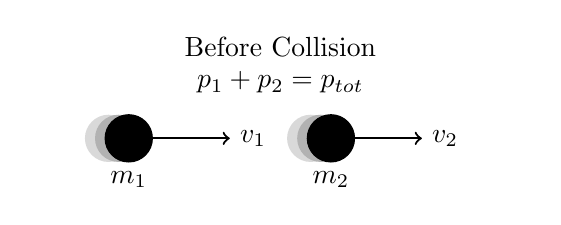
\begin{tikzpicture}
\begin{axis}[width=8cm, height=3cm,
    ticks=none,
    axis line style={draw=none},
    clip=false,
    xmin=0,xmax=10,
    ymin=0,ymax=10,
    title=Before Collision,
]
    \draw[thick,->] (2,5) -- ++(axis direction cs: 2,0) node[right] {$v_1$};
    \fill[black!15] (1.6,5) circle (3mm);
    \fill[black!30] (1.8,5) circle (3mm);
    \draw[fill=black] (2,5) circle (3mm) node[below=3mm] {$m_1$};
    \fill[black!15] (5.6,5) circle (3mm);
    \fill[black!30] (5.8,5) circle (3mm);
    \draw[thick,->] (6,5) -- ++(axis direction cs: 1.8,0) node[right] {$v_2$};
    \draw[fill=black] (6,5) circle (3mm) node[below=3mm] {$m_2$};
    \node at (5,10) {$p_1 + p_2 = p_{\text{tot}}$};
\end{axis}
\end{tikzpicture}%
\hspace{2em}
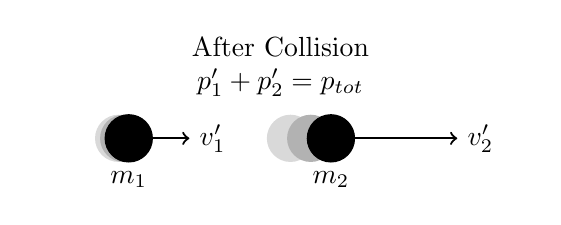
\begin{tikzpicture}
\begin{axis}[width=8cm, height=3cm,
    ticks=none,
    axis line style={draw=none},
    clip=false,
    xmin=0,xmax=10,
    ymin=0,ymax=10,
    title=After Collision,
]
    \draw[thick,->] (2,5) -- ++(axis direction cs: 1.2,0) node[right] {$v_1^{\prime}$};
    \fill[black!15] (1.8,5) circle (3mm);
    \fill[black!30] (1.9,5) circle (3mm);
    \draw[fill=black] (2,5) circle (3mm) node[below=3mm] {$m_1$};
    \fill[black!15] (5.2,5) circle (3mm);
    \fill[black!30] (5.6,5) circle (3mm);
    \draw[thick,->] (6,5) -- ++(axis direction cs: 2.5,0) node[right] {$v_2^{\prime}$};
    \draw[fill=black] (6,5) circle (3mm) node[below=3mm] {$m_2$};
    \node at (5,10) {$p_1^{\prime} + p_2^{\prime} = p_{\text{tot}}$};
\end{axis}
\end{tikzpicture}
\end{center}
\vspace{1em}

The result that momentum is conserved is true not only for this example involving the two cars but for any isolated system. An \gls{isolated system} is a system for which the net external force on the system is zero. The \gls{law of conservation of momentum} states that for an isolated system with any number of objects in it, the total momentum ($p_{\text{tot}}$) is conserved. In equation form, the law of conservation of momentum for an isolated system is written as

\begin{equation}
    p_{\text{tot}} = \text{constant}
\end{equation}

or

\begin{equation}
    p_{\text{tot}} = p_{\text{tot}}^{\prime}
\end{equation}

where $p_{\text{tot}}^{\prime}$ is the momentum of the system after a collision or event involving the constituent objects. In a two-object system, the law of conservation of momentum is

\begin{equation} \label{LgDXpb}
    p_1 + p_2 = p_1^{\prime} + p_2^{\prime}\ .
\end{equation}

Replacing $p$ with mass multiplied by velocity (see Eq.~\ref{L05jSw}), the law of conservation is 

\begin{equation} \label{eVkwoQ}
    m_1 v_1 + m_2 v_2 = m_1 v_1^{\prime} + m_2 v_2^{\prime}
\end{equation}

The conservation of momentum principle can be applied to systems as diverse as a comet striking the Earth or a gas containing huge numbers of atoms and molecules. Conservation of momentum appears to be violated only when the net external force is not zero. But another larger system can always be considered in which momentum is conserved by simply including the source of the external force. For example, in the collision of two cars considered above, the two-car system conserves momentum while each one-car system does not.

\begin{example} \label{W5BnBq} %%% Refer to this example at the beginning of the unit to motivate a better understanding of momentum. Our object is to scaffold up 
    Nancy the ice skater, whose mass is \SI{70}{kg}, stands at rest with ice skates on an icy (frictionless) surface. She uses superhero strength to throw a \SI{5}{kg} sack of potatoes horizontally away from her body at \SI{50}{m/s} (\SI{112}{mph}). As a result of both the frictionless surface and the law of conservation of momentum, she will accelerate in the direction opposite the sack. The speed she gains as a result throwing the object is known as the \textbf{recoil velocity}. Calculate Nancy's recoil velocity.
\end{example}

\begin{center}
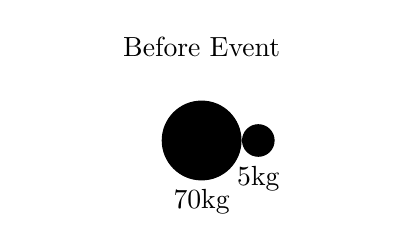
\begin{tikzpicture}
\begin{axis}[width=6cm,height=3.3cm,
    ticks=none,
    clip=false,
    xmin=-10,xmax=10,
    ymin=-4,ymax=3,
    axis line style={draw=none},
    title={Before Event},
]
    \draw[fill=black] (0,0) circle (5mm) node[below=5mm] {\SI{70}{kg}};
    \begin{scope}[xshift=7.2mm]
        \draw[fill=black] (0,0) circle (2mm) node[below=2mm] {\SI{5}{kg}};
    \end{scope}
\end{axis}
\end{tikzpicture}%
\hspace{1cm}
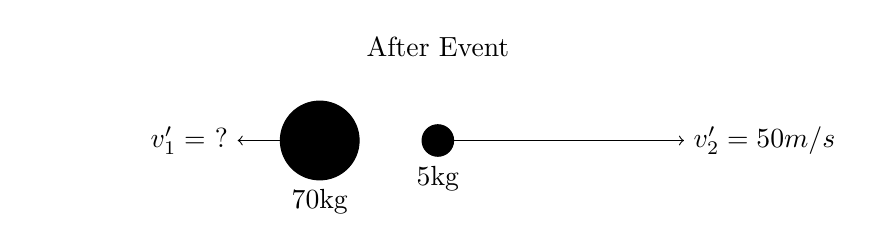
\begin{tikzpicture}
\begin{axis}[width=12cm,height=3.3cm,
    ticks=none,
    clip=false,
    xmin=-20,xmax=20,
    ymin=-4,ymax=3,
    title={After Event},
    axis line style={draw=none},
]
    \begin{scope}[xshift=-15mm]
        \draw[fill=black] (0,0) circle (5mm) node[below=5mm] {\SI{70}{kg}};
        \draw[->] (0,0) -- (-4,0) node[left] {$v_1^{\prime} =\ ?$};       
    \end{scope}
    \begin{scope}[xshift=0mm]
        \draw[fill=black] (0,0) circle (2mm) node[below=2mm] {\SI{5}{kg}};
        \draw[->] (0,0) -- (12,0) node[right] {$v_2^{\prime} = \SI{50}{m/s}$};
    \end{scope}
\end{axis}
\end{tikzpicture}
\end{center}

\Solution We are given Nancy's mass, the sack's mass, and the final velocity of the sack: $m_1 = \SI{70}{kg}$, $m_2 = \SI{5}{kg}$, and $v_2^{\prime} = \SI{50}{m/s}$. Furthermore, the initial velocities of both objects is zero: $v_1 = 0$ and $v_2 = 0$. The unknown quantity we're looking for is Nancy's final (recoil) velocity: $v_1^{\prime} =\ ?$ All these quantities are related by Equation \ref{eVkwoQ}, the law of conservation of momentum:

\begin{equation*}
    m_1 v_1 + m_2 v_2 = m_1 v_1^{\prime} + m_2 v_2^{\prime}
\end{equation*}

Substituting the known values leads to 

\begin{equation*}
    0 = 70\,v_1^{\prime} + (5)(50)
\end{equation*}

 which simplifies to 

 \begin{equation*}
     0 = 70\,v_1^{\prime} + 250
 \end{equation*}

 Solve for the recoil velocity ($v_1^{\prime}$) as follows:

 \begin{align*}
     \textbf{Write $v_1^{\prime}$ on left} \qquad & 70\,v_1^{\prime} + 250 = 0\\[0.5ex]
     \textbf{Subtract 250} \qquad & 70\,v_1^{\prime} + \cancel{250} \mathbin{\color{red} - } \textcolor{red}{\cancel{250}} = \mathbin{\color{red} - } \textcolor{red}{250}\\[0.5ex]
     \textbf{Simplify} \qquad &  70\,v_1^{\prime} = -250\\[0.5ex]
     \textbf{Divide by 70} \qquad & \frac{\cancel{70}\,v_1^{\prime}}{\textcolor{red}{\cancel{70}}} = \frac{-250}{\textcolor{red}{70}}\\[0.5ex]
     \textbf{Simplify} \qquad & v_1^{\prime} = -3.57\\
 \end{align*}

Therefore, Nancy's recoil velocity is \SI{-3.57}{m/s}. She slides backwards as a result of throwing the object forward, all while the momentum of the system remains conserved.
 
\endsolution


\subsection{Elastic Collisions} \label{vecM50}

When objects collide, they can either stick together or bounce off one another, remaining separate. In this section, we’ll cover these two different types of collisions.
\vspace{1em}

An \gls{elastic collision} is a collision in which objects separate after impact and the system doesn't lose any kinetic energy. (Kinetic energy is the energy of motion and is covered in the next unit.) The law of conservation of momentum is very useful here, and it can be used whenever the net external force on a system is zero. 
%Figure 8.6 shows an elastic collision where momentum is conserved.
\vspace{1em}

\begin{center}
\def\xa{1.5}
\def\xb{8.5}
\def\y{3}
\def\rb{6mm}
\begin{tikzpicture}
\begin{axis}[width=8cm, height=3cm,
    ticks=none,
    axis line style={draw=none},
    clip=false,
    xmin=0,xmax=10,
    ymin=0,ymax=10,
    title=Before Collision,
]
    \draw[thick,->] (\xa,\y) -- ++(axis direction cs: 3,0) node[right] {$v_1$};
    \fill[black!15] (\xa-0.3,\y) circle (3mm);
    \fill[black!30] (\xa-0.15,\y) circle (3mm);
    \draw[fill=black] (\xa,\y) circle (3mm) node[below=3mm] {$m_1$};
    \fill[black!15] (\xb+0.3,\y) circle (\rb);
    \fill[black!30] (\xb+0.15,\y) circle (\rb);
    \draw[thick,->] (\xb,\y) -- ++(axis direction cs: -2,0) node[left] {$v_2$};
    \draw[fill=black] (\xb,\y) circle (\rb) node[below=\rb] {$m_2$};
    \node at (5,10) {$p_1 + p_2 = p_{\text{tot}}$};
\end{axis}
\end{tikzpicture}%
\hspace{2em}
\def\xa{3.5}
\def\xb{6.5}
\def\y{3}
\def\rb{6mm}
\begin{tikzpicture}
\begin{axis}[width=8cm, height=3cm,
    ticks=none,
    axis line style={draw=none},
    clip=false,
    xmin=0,xmax=10,
    ymin=0,ymax=10,
    title=After Collision,
]
    \draw[thick,->] (\xa,\y) -- ++(axis direction cs: -4,0) node[left] {$v_1^{\prime}$};
    \fill[black!15] (\xa+0.4,\y) circle (3mm);
    \fill[black!30] (\xa+0.2,\y) circle (3mm);
    \draw[fill=black] (\xa,\y) circle (3mm) node[below=3mm] {$m_1$};
    \fill[black!15] (\xb-0.24,\y) circle (\rb);
    \fill[black!30] (\xb-0.12,\y) circle (\rb);
    \draw[thick,->] (\xb,\y) -- ++(axis direction cs: 1.5,0) node[right] {$v_2^{\prime}$};
    \draw[fill=black] (\xb,\y) circle (\rb) node[below=\rb] {$m_2$};
    \node at (5,10) {$p_1^{\prime} + p_2^{\prime} = p_{\text{tot}}$};
\end{axis}
\end{tikzpicture}
\end{center}

Perfectly elastic collisions can happen only with subatomic particles. Everyday observable examples of perfectly elastic collisions don't exist---some kinetic energy is always lost, as it is converted into heat transfer due to friction. However, collisions between everyday objects are \textit{almost} perfectly elastic when they occur with objects and surfaces that are nearly frictionless, such as with two steel blocks on ice. Thus, we may assume that all examples and exercises covered hereafter are perfectly elastic.
\vspace{1em}

For problems involving one-dimensional elastic collisions between two objects, we can use the same equation for conservation of momentum, which we labeled Equation (\ref{LgDXpb}):

\begin{equation*}
    p_1 + p_2 = p_1^{\prime} + p_2^{\prime}
\end{equation*}

Previously, we said that this equation is equivalent to Equation (\ref{eVkwoQ}):

\begin{equation*} 
    m_1 v_1 + m_2 v_2 = m_1 v_1^{\prime} + m_2 v_2^{\prime}
\end{equation*}

where the primes $\left(\,^{\prime}\,\right)$ indicate values after the collision. The equation assumes that the mass of each object does not change during the collision.

\begin{example} \label{wXY1rT}
    An object with a mass of \SI{0.9}{kg} moving at \SI{1.0}{m/s} experiences an elastic collision with an object of mass \SI{1.5}{kg} moving at \SI{-0.5}{m/s}. If the first object's velocity after collision is \SI{-0.88}{m/s}, what is the second object's velocity?
\end{example}

\begin{center}
\def\xa{1.5}
\def\xb{8.5}
\def\y{3}
\def\ra{4mm}
\def\rb{6mm}
\begin{tikzpicture}
\begin{axis}[width=8cm, height=3cm,
    ticks=none,
    axis line style={draw=none},
    clip=false,
    xmin=0,xmax=10,
    ymin=0,ymax=10,
    title=Before Collision,
]
    \draw[thick,->] (\xa,\y) -- ++(axis direction cs: 3,0) node[above] {$\SI{1.0}{m/s}$};
    \fill[black!15] (\xa-0.3,\y) circle (\ra);
    \fill[black!30] (\xa-0.15,\y) circle (\ra);
    \draw[fill=black] (\xa,\y) circle (\ra) node[below=\ra] {$\SI{0.9}{kg}$};
    \fill[black!15] (\xb+0.3,\y) circle (\rb);
    \fill[black!30] (\xb+0.15,\y) circle (\rb);
    \draw[thick,->] (\xb,\y) -- ++(axis direction cs: -1.8,0); \node at (6.4,1) {$\SI{-0.5}{m/s}$};
    \draw[fill=black] (\xb,\y) circle (\rb) node[below=\rb] {$\SI{1.5}{kg}$};
    \node at (5,10) {$p_1 + p_2 = p_{\text{tot}}$};
\end{axis}
\end{tikzpicture}%
\hspace{2em}
\def\xa{3.5}
\def\xb{6.5}
\def\y{3}
\def\ra{4mm}
\def\rb{6mm}
\begin{tikzpicture}
\begin{axis}[width=8cm, height=3cm,
    ticks=none,
    axis line style={draw=none},
    clip=false,
    xmin=0,xmax=10,
    ymin=0,ymax=10,
    title=After Collision,
]
    \draw[thick,->] (\xa,\y) -- ++(axis direction cs: -2.8,0) node[left] {$\SI{-0.88}{m/s}$};
    \fill[black!15] (\xa+0.4,\y) circle (\ra);
    \fill[black!30] (\xa+0.2,\y) circle (\ra);
    \draw[fill=black] (\xa,\y) circle (\ra) node[below=\ra] {$\SI{0.9}{kg}$};
    \fill[black!15] (\xb-0.24,\y) circle (\rb);
    \fill[black!30] (\xb-0.12,\y) circle (\rb);
    \draw[thick,->] (\xb,\y) -- ++(axis direction cs: 2.3,0) node[right] {$v_2^{\prime} =\ ?$};
    \draw[fill=black] (\xb,\y) circle (\rb) node[below=\rb] {$\SI{1.5}{kg}$};
    \node at (5,10) {$p_1^{\prime} + p_2^{\prime} = p_{\text{tot}}$};
\end{axis}
\end{tikzpicture}
\end{center}

\Solution We are given the masses and initial velocities of both objects and the velocity after collision of the first object: $m_1 = \SI{0.9}{kg}$, $v_1 = \SI{1.0}{m/s}$, $m_2 = \SI{1.5}{kg}$, $v_2 = \SI{-0.5}{m/s}$, and $v_1^{\prime} = \SI{-0.88}{m/s}$. The unknown we want to find is the velocity of the second object after collision: $v_2^{\prime} =\ ?$. These variables are all related by Eq.~(\ref{eVkwoQ}), the conservation of momentum equation:

\begin{equation*} 
    m_1 v_1 + m_2 v_2 = m_1 v_1^{\prime} + m_2 v_2^{\prime}
\end{equation*}

Substituting the given values leads to

\begin{equation*}
    (0.9)(1) + (1.5)(-0.5) = (0.9)(-0.88) + (1.5) v_2^{\prime}\ ,
\end{equation*}

which reduces to

\begin{equation*}
    0.15 = -0.792 + 1.5\,v_2^{\prime}
\end{equation*}

We solve this equation for $v_2^{\prime}$ via the following steps:
\vspace{-1em}

\begin{align*}
    \textbf{Write $v_2^{\prime}$ on left} \qquad & 1.5\,v_2^{\prime} - 0.792 = 0.15\\[1ex]
    \textbf{Add 0.792} \qquad & 1.5\,v_2^{\prime} - \cancel{0.792} \redplus \textcolor{red}{\cancel{0.792}} = 0.15 \redplus \textcolor{red}{0.792}\\[1ex]
    \textbf{Reduce} \qquad & 1.5\,v_2^{\prime} = 0.942\\[1ex]
    \textbf{Divide by 1.5} \qquad & \frac{\cancel{1.5}\,v_2^{\prime}}{\textcolor{red}{\cancel{1.5}}} = \frac{0.942}{\textcolor{red}{1.5}}\\[1ex]
    \textbf{Reduce} \qquad & v_2^{\prime} = 0.628
\end{align*}

Therefore, the velocity of the second object after collision is (rounding up) $v_2^{\prime} = +\SI{0.63}{m/s}$.

\endsolution

\cyanhrule

\subsection{Inelastic Collisions} \label{v90mza}

Next, we turn to the second type of collision. An \gls{inelastic collision} is one in which objects stick together after impact, and kinetic energy of the system is not conserved. This lack of conservation means that the forces between colliding objects may convert kinetic energy to other forms of energy, such as potential energy or thermal energy. (Again, the concepts of energy are discussed more thoroughly in the next unit). For inelastic collisions, kinetic energy may be lost in the form of heat. 
\vspace{1em}

The figure below shows an example of an inelastic collision. Two objects head toward each other and then stick together. After sticking together, momentum is conserved but not kinetic energy. Some of the energy of motion gets converted to thermal energy, or heat.

\begin{center}
\def\xa{1.5}
\def\xb{8.5}
\def\y{3}
\def\rb{6mm}
\begin{tikzpicture}
\begin{axis}[width=8cm, height=3cm,
    ticks=none,
    axis line style={draw=none},
    clip=false,
    xmin=0,xmax=10,
    ymin=0,ymax=10,
    title=Before Collision,
]
    \draw[thick,->] (\xa,\y) -- ++(axis direction cs: 3,0) node[right] {$v_1$};
    \fill[black!15] (\xa-0.3,\y) circle (3mm);
    \fill[black!30] (\xa-0.15,\y) circle (3mm);
    \draw[fill=black] (\xa,\y) circle (3mm) node[below=3mm] {$m_1$};
    \fill[black!15] (\xb+0.3,\y) circle (\rb);
    \fill[black!30] (\xb+0.15,\y) circle (\rb);
    \draw[thick,->] (\xb,\y) -- ++(axis direction cs: -2,0) node[left] {$v_2$};
    \draw[fill=black] (\xb,\y) circle (\rb) node[below=\rb] {$m_2$};
    \node at (5,10) {$p_1 + p_2 = p_{\text{tot}}$};
\end{axis}
\end{tikzpicture}%
\hspace{2em}
\def\xa{4.3}
\def\xb{5.7}
\def\y{3}
\def\rb{6mm}
\begin{tikzpicture}
\begin{axis}[width=8cm, height=3cm,
    ticks=none,
    axis line style={draw=none},
    clip=false,
    xmin=0,xmax=10,
    ymin=0,ymax=10,
    title=After Collision,
]
    \draw[thick,->] (\xa,\y) -- ++(axis direction cs: -1.2,0) node[left] {$v^{\prime}$};
    \draw[fill=black] (\xa,\y) circle (3mm) node[below=3mm] {$m_1$};
    \fill[black!15] (\xb+0.2,\y) circle (\rb);
    \fill[black!30] (\xb+0.1,\y) circle (\rb);
    \draw[fill=black] (\xb,\y) circle (\rb) node[below=\rb] {$m_2$};
    \node at (5,10) {$p_1^{\prime} + p_2^{\prime} = p_{\text{tot}}$};
\end{axis}
\end{tikzpicture}
\end{center}

Since the two objects stick together after colliding, they move together at the same speed. In such a case, the conservation of momentum equation (Eq.~\ref{eVkwoQ}),
\vspace{-1ex}

\begin{equation*}
    m_1 v_1 + m_2 v_2 = m_1 v_1^{\prime} + m_2 v_2^{\prime}\ ,
\end{equation*}

becomes

\begin{equation} \label{6HFSQ5}
    m_1 v_1 + m_2 v_2 = (m_1 + m_2)\,v^{\prime}
\end{equation}

 
for inelastic collisions, where $v^{\prime}$ is the final velocity for both objects as they are stuck together.

\begin{example}\label{usQeew}
    A \SI{0.500}{kg} object that is moving at a velocity of \SI{1.00}{m/s} inelastically collides with a \SI{1.50}{kg} object that is moving at \SI{-0.500}{m/s}. What is the final velocity of the combined system after the collision?
\end{example}

\begin{center}
\def\xa{1.5}
\def\xb{8.5}
\def\y{3}
\def\rb{6mm}
\begin{tikzpicture}
\begin{axis}[width=8cm, height=3cm,
    ticks=none,
    axis line style={draw=none},
    clip=false,
    xmin=0,xmax=10,
    ymin=0,ymax=10,
    title=Before Collision,
]
    \draw[thick,->] (\xa,\y) -- ++(axis direction cs: 3,0) node[above] {$\SI{+1.0}{m/s}$};
    \fill[black!15] (\xa-0.3,\y) circle (3mm);
    \fill[black!30] (\xa-0.15,\y) circle (3mm);
    \draw[fill=black] (\xa,\y) circle (3mm) node[below=3mm] {$\SI{0.5}{kg}$};
    \fill[black!15] (\xb+0.3,\y) circle (\rb);
    \fill[black!30] (\xb+0.15,\y) circle (\rb);
    \draw[thick,->] (\xb,\y) -- ++(axis direction cs: -2.2,0) node[below] {$\SI{-0.5}{m/s}$};
    \draw[fill=black] (\xb,\y) circle (\rb) node[below=\rb] {$\SI{1.5}{kg}$};
    \node at (5,10) {$p_1 + p_2 = p_{\text{tot}}$};
\end{axis}
\end{tikzpicture}%
\hspace{2em}
\def\xa{4.3}
\def\xb{5.7}
\def\y{3}
\def\rb{6mm}
\begin{tikzpicture}
\begin{axis}[width=8cm, height=3cm,
    ticks=none,
    axis line style={draw=none},
    clip=false,
    xmin=0,xmax=10,
    ymin=0,ymax=10,
    title=After Collision,
]
    \draw[thick,->] (\xa,\y) -- ++(axis direction cs: -1.2,0) node[left] {$v^{\prime}$};
    \draw[fill=black] (\xa,\y) circle (3mm);
    \fill[black!15] (\xb+0.2,\y) circle (\rb);
    \fill[black!30] (\xb+0.1,\y) circle (\rb);
    \draw[fill=black] (\xb,\y) circle (\rb);
    \node at (5,10) {$p_1^{\prime} + p_2^{\prime} = p_{\text{tot}}$};
    \node at (5,-3) {\SI{2.0}{kg}};
\end{axis}
\end{tikzpicture}
\end{center}



\Solution We are given two masses and two initial velocities: $m_1 = \SI{0.5}{kg}$, $m_2 = \SI{1.5}{kg}$, $v_1 = \SI{+1.0}{m/s}$, and $v_2 = \SI{-0.5}{m/s}$.  We want to find the final velocity of the stuck system: $v^{\prime} =\ ?$. These quantities are related by Equation~(\ref{6HFSQ5}) for inelastic collisions:
\vspace{-1ex}

\begin{equation*}
    m_1 v_1 + m_2 v_2 = (m_1 + m_2)\,v^{\prime}
\end{equation*}

To solve this equation for $v^{\prime}$, we take the following steps:
\vspace{-1ex}

\begin{align*}
    \textbf{Substitute given values} \qquad & (0.5)(1.0) + (1.5)(-0.5) = (0.5 + 1.5)\,v^{\prime}\\[1ex]
    \textbf{Simplify} \qquad & -0.25 = 2\,v^{\prime}\\[1ex]
    \textbf{Write $v^{\prime}$ on left} \qquad & 2\,v^{\prime} = -0.25\\[1ex]
    \textbf{Divide by 2} \qquad & \frac{\cancel{2}\,v^{\prime}}{\textcolor{red}{\cancel{2}}} = \frac{-0.25}{\textcolor{red}{\cancel{2}}}\\[1ex]
    \textbf{Simplify} \qquad & v^{\prime} = -\SI{0.125}{m/s}
\end{align*}

Therefore, the final velocity of the system is (rounding up) \SI{-0.13}{m/s}; the system moves leftward.

\cyanhrule

\begin{mdframed}[backgroundcolor=black!10]
\textbf{How to Remember Elastic vs.~Inelastic}
\vspace{1ex}

Here's a mnemonic to help you remember the difference between elastic and inelastic collisions: When \href{https://youtu.be/UOyDnrAZmhA?t=14}{Chas McCormick} catches a baseball with his glove, the ball and glove collide and stick together. Where is the ball? It's \underline{\textbf{in}} the glove; this is an \underline{\textbf{in}}elastic collision---one in which objects stick together. Then you can remember that if they don't stick together, the collision must be elastic.
\end{mdframed}


\clearpage
\printnoidxglossaries

\clearpage

\subsection{Work} \label{obMgG8}

In physics, the term work has a very specific definition. \Gls{work} is the product of force and distance such that an object experiencing the force moves by that distance. Mathematically, work is force multiplied by distance:

\begin{equation} \label{y0Z6Cw}
    W = F d
\end{equation}

\begin{center}
    \begin{tabular}{cl|cl}
    \hline
    \textbf{Symbol} & \textbf{Quantity} & \textbf{SI Base Unit} & \textbf{Unit Symbol}  \\
    \hline\hline
    \rule{0pt}{2.5ex}
        $W$ & work & joule & J\\
        $F$ & force & newton & N\\
        $d$ & distance & meter & m\\
    \hline
    \end{tabular}
\end{center}

The \gls{joule} (J) is the metric unit for work and energy and is equal to 1 newton-meter (N$\cdot$m):

\begin{center}
    1 Joule (J) $=$ 1 Newton $\!\cdot\!$ meter (\SI{}{N\!\cdot\!m})
\end{center}

Some things that we typically consider to be work are not work in the scientific sense of the term. Let's consider a few examples. Think about why each of the following statements is true.

\begin{itemize}
\setlength\itemsep{-0.8ex}
    \item Homework \textit{is not} work.
    \item Lifting a rock upwards off the ground \textit{is} work.
    \item Carrying a rock in a straight path across the lawn at a constant speed \textit{is not} work.
\end{itemize}

The first two examples are fairly simple. Homework is not work because objects are not being moved over a distance. Lifting a rock up off the ground is work because the rock is moving in the direction that force is applied. The last example is less obvious. Recall from the laws of motion that force is not required to move an object at constant velocity. Therefore, while some force may be applied to keep the rock up off the ground, no net force is applied to keep the rock moving forward at constant velocity.

\begin{example} \label{HKavsZ}
Jacob applies a force of \SI{72.0}{N} on a box and pushes it a distance of \SI{25.0}{m}. How much work is done on the box?
\end{example}

\begin{center}
    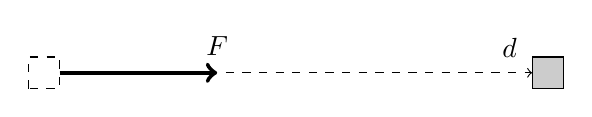
\begin{tikzpicture}

    \begin{scope}[xshift=-4mm,yshift=-2mm]
        \draw[dashed] (0,0) rectangle (4mm,4mm);
    \end{scope}

    \begin{scope}[xshift=6cm,yshift=-2mm]
        \draw[fill=black!20] (0,0) rectangle (4mm,4mm);
    \end{scope}
    
    \draw[ultra thick, ->] (0,0) -- (2,0) node[above=2pt] {$F$};
    \draw[->, dashed] (0,0) -- (6,0) node[above left=2pt] {$d$};
    \end{tikzpicture}
\end{center}

\Solution We are given the quantities of force and distance: $F = \SI{72.0}{N}$ and $d = \SI{25.0}{m}$. The unknown quantity we want to find is work. By Equation~(\ref{y0Z6Cw}), 

\begin{equation*}
    W = F d = \left(\SI{72.0}{N}\right)\left(\SI{25.0}{m}\right) = \SI{1800}{J}
\end{equation*}

Jacob does 1800 joules of work on the box in applying the force to move the box.

\cyanhrule

\begin{example} \label{O9RxyJ}
You see a box with a mass of \SI{10}{kg} resting on the floor. What is the work you have to do on the box to lift it to a height of 1.5 meters? (This example is like the vertical version of Example \ref{HKavsZ}.)
\end{example} 


\Solution We are given the box's mass and distance lifted: $m = \SI{10}{kg}$ and $d = \SI{1.5}{m}$. The unknown we are looking for is work: $W =\ ?$ By Eq.~(\ref{y0Z6Cw}), work is

\begin{equation*}
    W = F d
\end{equation*}

However, force ($F$) is \textit{not} one of the given quantities in this problem. Can you of a way to calculate how much force is necessary to lift this box? To lift the box, you must supply an upward force that is (at least) equal to the magnitude of the downward force of gravity on the box. That is, your applied force must equal the box's weight ($w$), which, in Unit 4 on Forces, we specifically defined as

\begin{equation*}
    w = m g\ ,
\end{equation*}

where  g = \SI{9.8}{m/s^2}. So, if your applied force is equal to the box's weight, then your force is

\begin{equation*}
    F = w = mg = (10)(9.8) = \SI{98}{N}
\end{equation*}

Therefore, the work done is

\begin{equation*}
    W = F d = (\SI{98}{N})(\SI{1.5}{m}) = \SI{147}{J} \ .
\end{equation*}

\textbf{Note}: Since, in this example, the force was of the form $F = mg$ and since work is defined as $W = F d$, the work done against gravity was of the form $W = mgd$. Compare this result with Equation (\ref{RlpJa5}) below.

\cyanhrule

\subsection{Power} \label{bxZysw}

In applications that involve work, we are often interested in how fast the work is done. For example, in roller coaster design, the amount of time it takes to lift a roller coaster car to the top of the first hill is an important consideration. Taking a half hour on the ascent will surely irritate riders and decrease ticket sales. Let's take a look at how to calculate the time it takes to do work.
\vspace{1em}

Recall that a rate can be used to describe a quantity, such as work, over a period of time. \Gls{power} is the rate at which work is done. In this case, rate means per unit of time. Power is calculated by dividing the work done by the time it took to do the work.

\begin{equation} \label{k6uV1p}
    P = \frac{W}{t}
\end{equation}

\begin{center}
    \begin{tabular}{cl|cl}
    \hline
    \textbf{Symbol} & \textbf{Quantity} & \textbf{SI Base Unit} & \textbf{Unit Symbol}  \\
    \hline\hline
    \rule{0pt}{2.5ex}
        $P$ & power & watt & W\\
        $W$ & work & joule & J\\
        $t$ & time & second & s\\
    \hline
    \end{tabular}
\end{center}


Let's consider an example that can help illustrate the differences among work, force, and power. Suppose the woman in the figure to the right lifting the TV with a pulley gets the TV to the fourth floor in two minutes, and the man carrying the TV up the stairs takes five minutes to arrive at the same place. They have done the same amount of work ($F d$) on the TV, because they have moved the same mass over the same vertical distance, which requires the same amount of upward force. However, the woman using the pulley has generated more power. This is because she did the work in a shorter amount of time, so the denominator of the power formula, $t$, is smaller.



Power can be expressed in units of watts (W). This unit can be used to measure power related to any form of energy or work. You have most likely heard the term used in relation to electrical devices, especially light bulbs. Multiplying power by time gives the amount of energy. Electricity is sold in kilowatt-hours because that equals the amount of electrical energy consumed. The watt unit was named after James Watt (1736--1819). He was a Scottish engineer and inventor who discovered how to coax more power out of steam engines.

\vspace{1em}

\cyanhrule

\subsection{Energy} \label{iHOPFl}

\Gls{energy} is defined as the ability to do work. Energy is a measure of how much change can happen in a system, like a change in motion or a change in conditions such as shape, temperature, or composition. Work and energy are closely related. When you do work to move an object, you change the object's energy. You (or an object) also expend energy to do work. Energy can take a variety of different forms, and one form of energy can transform to another. In this chapter we will be concerned with \gls{mechanical energy}, which comes in two forms: kinetic energy and potential energy.

\begin{itemize}
\setlength\itemsep{-0.8ex}
    \item \Gls{kinetic energy} is also called energy of motion. A moving object has kinetic energy.
    \item \Gls{potential energy}, sometimes called stored energy, comes in several forms. \Gls{gravitational potential energy} is the stored energy an object has as a result of its position above Earth's surface (or another object in space). A roller coaster car at the top of a hill has gravitational potential energy.
\end{itemize}

Like work, the SI unit of energy is the joule (J).

\vspace{1em}

\cyanhrule


\subsection{Gravitational Potential Energy} \label{vRflRn}

In Example \ref{O9RxyJ}, work was done against gravity, an action which merits special recognition in physics.

% \colorbox{yellow}{\textbf{Potential energy}} is energy that is stored.

\Gls{gravitational potential energy} ($\mathrm{PE_g}$) is energy that is stored by doing \textbf{work} against gravity.

\begin{center}
\def\height{3}
\begin{tikzpicture}
\begin{axis}[width=8cm,height=5cm,
    clip=false,
    ticks=none,
    xmin=-2,xmax=3,ymin=-0.5,ymax=3.5,
    axis lines=center,
    axis line style={draw=none}
]
\draw[->] (-1,0) -- ++(axis direction cs: 0,\height) node[right=2pt] {$h$};
\fill (0,\height) circle (3pt) node[right=2pt] {$m$};
\draw[->,thick] (0,\height) -- ++(axis direction cs: 0,-1); %node[below] {\footnotesize weight};
\draw[->,dashed,thick] (1,0) -- ++(axis direction cs: 0,\height) node[right=2pt] {$\mathrm{PE_g}$};
\draw (-2,0) -- (2,0);
\node at (0,-0.3) {reference level: $\mathrm{PE_g} = 0$};
\end{axis}
\end{tikzpicture}
\end{center}

The equation for gravitational potential energy is

\begin{equation} \label{RlpJa5}
    \mathrm{PE_g} = mgh
\end{equation}

where $h$ is the height above the reference point at which potential energy is zero, and where where $g = \SI{9.8}{m/s}$ for object near the surface of Earth. Change in $\mathrm{PE_g}$ is then

\begin{equation} 
    \Delta\mathrm{PE_g} = m g\,\Delta h\ ,
\end{equation}

\begin{center}
    \begin{tabular}{cl|cl}
    \hline
    \textbf{Symbol} & \textbf{Quantity} & \textbf{SI Base Unit} & \textbf{Unit Symbol}  \\
    \hline\hline
    \rule{0pt}{2.5ex}
        $\mathrm{PE_g}$ & gravitational potential energy & joule & J\\
        $m$ & mass & kilogram & kg\\
        $g$ & acceleration due to gravity & meter per second squared & \SI{}{m/s^2}\\
        $h$ & height & meter & m\\
    \hline
    \end{tabular}
\end{center}

\cyanhrule

\begin{example} \label{J1Qehp}
A 2.0-kg ball gets kicked in the air to a maximum height of 15 meters. At the peak height, what is the gravitational potential energy of the ball?
\end{example}

\Solution We are given mass and height: $m = \SI{2.0}{kg}$, $h = \SI{15}{m}$, and gravity is $\SI{9.8}{m/s^2}$. The unknown we are finding in gravitational potential energy: $\mathrm{PE_g} =\ ?$ By Eq.~(\ref{RlpJa5}),

\begin{equation*}
    \mathrm{PE_g} = m g h = (2.0)(9.8)(15) =  \SI{294}{J} \ .
\end{equation*}

\cyanhrule

% \textit{YouTube}: ``Chris Farley -- Greatest Entrance Ever'' by MyTalkShowHeroes (\href{https://youtu.be/_z9kdqDwA80}{link}). Watch the first 1:00 min. What does Chris Farley have a lot of? Energy. More specifically, kinetic energy.

\clearpage
% Kinetic energy moved to unit 1!!!

\subsection{Conservation of Mechanical Energy} \label{KRxiCV}

\Gls{mechanical energy} is the sum of kinetic energy and potential energy. The law of conservation of mechanical energy says that for a closed system energy is conserved. This law is expressed as

\begin{equation} \label{QyLUh5}
    \mathrm{ME} = \mathrm{KE} + \mathrm{PE} = \mathrm{constant}
\end{equation}

but is more usefully written as

\begin{equation} \label{yOUj22}
    \mathrm{KE_i} + \mathrm{PE_i} = \mathrm{KE_f} + \mathrm{PE_f}
\end{equation}


If we replace each $\mathrm{KE}$ and $\mathrm{PE}$ with the forms in Equations (\ref{s57crz}) and (\ref{RlpJa5}), the law of conservation of energy becomes

\begin{equation} \label{ZSmSin}
    \frac{1}{2} m v_i^2 + mgh_i  = 
    \frac{1}{2} m v_f^2 + mgh_f 
\end{equation}

\begin{example} \label{mUfgIz}
Tony Hawk starts from rest from the top of a 6-meter tall ramp. His mass is \SI{77}{kg}. What will be his kinetic energy at the bottom of the ramp? Assume no energy is lost to friction.
\end{example}

\begin{center}
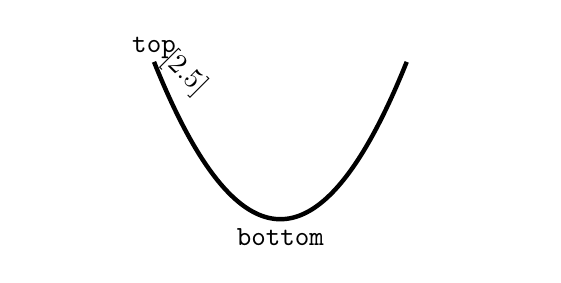
\begin{tikzpicture}
\begin{axis}[width=8cm,height=3.5cm,
    clip=false,
    xmin=-5,xmax=5,ymin=0,ymax=6,
    axis lines=center,
    axis line style={draw=none},
    ticks=none,
]
\addplot[ultra thick,samples=100,
    domain=-2.5:2.5
]{x^2}; 
\node[below] at (0,0) {\texttt{bottom}};
\node[above] at (-2.5,6) {\texttt{top}};
\node[rotate=-45] at (-1.9,5.8) {\Strichmaxerl[2.5]};
\end{axis}
\end{tikzpicture}
\end{center}

\Solution By the law of conservation of mechanical energy (Eq.~\ref{yOUj22}), Hawk's mechanical energy is governed by the equation

\begin{equation*} 
    \mathrm{KE_i} + \mathrm{PE_i} = \mathrm{KE_f} + \mathrm{PE_f}
\end{equation*}

At the top, Hawk has no motion, so his initial kinetic energy is zero: $\mathrm{KE_i} = 0$. At the bottom, he loses all height above the ramp, so his gravitational potential energy is zero: $\mathrm{PE_f} = 0$. Therefore, conservation of energy reduces from

\begin{equation*}
        \cancel{\mathrm{KE_i}} + \mathrm{PE_i} = \mathrm{KE_f} + \cancel{\mathrm{PE_f}}
\end{equation*}

to

\begin{equation} \label{eosZpi}
    \mathrm{PE_i} = \mathrm{KE_f}
\end{equation}

This result means that all of Hawk's potential (stored) energy at the top of the ramp will be converted to kinetic (motion) energy when he reaches the bottom.
\vspace{1em}

We are given Hawk's mass and his initial height above the ramp: $m = \SI{77}{kg}$ and $h_i = \SI{6}{m}$. The unknown we're looking for is his final kinetic energy, at the bottom of the ramp: $\mathrm{KE_f} =\ ?$ The given quantities are related by Eq.~(\ref{RlpJa5}), which provides Hawk's initial gravitational potential energy:

\begin{equation*}
    \mathrm{PE_i} = mgh_i = (77)(9.8)(6) = \SI{4527.6}{J} 
\end{equation*}

This energy, by Eq.~(\ref{eosZpi}), gets converted to Hawk's kinetic energy, so

\begin{equation*}
    \mathrm{KE_f} = \SI{4527.6}{J} 
\end{equation*}

This example is to show that all of Tony Hawk's gravitational potential energy at the top of the ramp was entirely converted to his kinetic energy at the bottom.

\endsolution

\vspace{1em}

\cyanhrule

\begin{example} \label{nQVUKM}
    When Tony Hawk reaches the bottom, in Example \ref{mUfgIz}, what is his speed?
\end{example}

\Solution At the end of Example \ref{mUfgIz} we concluded that his kinetic energy at the bottom is 

\begin{equation*}
    \mathrm{KE_f} = \SI{4527.6}{J}
\end{equation*}

But by Eq.~(\ref{s57crz}), his kinetic energy is

\begin{equation*}
    \mathrm{KE} = \frac{1}{2} m v^2
\end{equation*}

Substituting the given values leads to 

\begin{equation*}
    4527.6 = \frac{1}{2} \cdot 77 \cdot v^2
\end{equation*}

If we solve this equation for speed ($v$), as we did in Example \ref{PUlJG6}, then his speed is

\begin{equation*}
    v = \SI{10.8}{m/s}
\end{equation*}

\cyanhrule


\subsection{Advanced Topics (AP Physics Students Only)} 

The laws of conservation of momentum and energy are

\begin{equation} \label{EFyWT6}
    m_1 v_1 + m_2 v_2 = m_1 v_1^{\prime} + m_2 v_2^{\prime}
\end{equation}

\begin{equation*}
    \frac{1}{2} m_1 v_1^2 + \frac{1}{2} m_2 v_2^2 = \frac{1}{2} m_1 v_1^{\prime\,2} + \frac{1}{2} m_2 v_2^{\prime\,2}
\end{equation*}

Note that the $\frac{1}{2}$ cancels in all terms in the above equation, leading to

\begin{equation} \label{jPL9Aw}
    m_1 v_1^2 + m_2 v_2^2 = m_1 v_1^{\prime\,2} + m_2 v_2^{\prime\,2}
\end{equation}

Eq.~(\ref{EFyWT6}) is solved for $v_2^{\prime}$ as

\begin{equation} \label{7OTaEl}
    v_2^{\prime} = \frac{m_1}{m_2} \left(v_1 - v_1^{\prime}\right) + v_2
\end{equation}

Let 

\begin{equation*}
    \alpha = \frac{m_1}{m_2} \left(v_1 - v_1^{\prime}\right)\ , \quad 
    \beta = v_2
\end{equation*}

Then

\begin{equation} \label{HN7pyf}
    v_2^{\prime\,2} = (\alpha + \beta)^2 = \frac{m_1^2}{m_2^2} \left(v_1^2 - 2v_1 v_1^{\prime} + v_1^{\prime\,2}\right) +
    \frac{2 m_1}{m_2} \left(v_1 - v_1^{\prime}\right) v_2 + v_2^2
\end{equation}



Eq.~(\ref{HN7pyf}) implies that the $m_2 v_2^{\prime\,2}$ term from Eq.~(\ref{jPL9Aw}) is

\begin{equation*}
    m_2 v_2^{\prime\,2} = \frac{m_1^2}{m_2} \left(v_1^2 - 2v_1 v_1^{\prime} + v_1^{\prime\,2}\right) +
    2m_1 \left(v_1 - v_1^{\prime}\right) v_2 + m_2 v_2^2
\end{equation*}

which may be distributed as

\begin{equation} \label{8hdEtk}
    m_2 v_2^{\prime\,2} = \left(\frac{m_1^2}{m_2}\right) v_1^2 - \left(\frac{2m_1^2}{m_2}\right) v_1 v_1^{\prime} + \left(\frac{m_1^2}{m_2}\right) v_1^{\prime\,2} + 2m_1 v_1 v_2 - 2 m_1 v_2 v_1^{\prime} + m_2 v_2^2
\end{equation}

Let $\gamma = m_1/m_2$. Then for convenience we can write Eq.~(\ref{8hdEtk}) as

\begin{equation} \label{8dhad6}
    m_2 v_2^{\prime\,2} = \gamma\, m_1 v_1^2 - 2 m_1 \left(\gamma\, v_1 + v_2\right)v_1^{\prime} + \gamma\, m_1 v_1^{\prime\,2} + 2m_1 v_1 v_2 + m_2 v_2^2
\end{equation}

Plugging Eq.~(\ref{8dhad6}) back into Eq.~(\ref{jPL9Aw}) leads to 

\begin{equation*}
    m_1 v_1^2 + \cancel{m_2 v_2^2} = m_1 v_1^{\prime\,2} + \gamma\, m_1 v_1^2 - 2 m_1 \left(\gamma\, v_1 + v_2\right)v_1^{\prime} + \gamma\, m_1 v_1^{\prime\,2} + 2m_1 v_1 v_2 + \cancel{m_2 v_2^2}
\end{equation*}

which may be rearranged to the quadratic form

% \begin{equation*}
%     m_1 v_1^2 = m_1 v_1^{\prime\,2} + \gamma\, m_1 v_1^2 - 2 m_1 \left(\gamma\, v_1 + v_2\right)v_1^{\prime} + \gamma\, m_1 v_1^{\prime\,2} + 2m_1 v_1 v_2 
% \end{equation*}

% \begin{equation*}
%     m_1 v_1^2 = (\gamma + 1) m_1 v_1^{\prime\,2}  - 2 m_1 \left(\gamma\, v_1 + v_2\right)v_1^{\prime} + \gamma\, m_1 v_1^2 + 2m_1 v_1 v_2 
% \end{equation*}

\begin{equation} \label{xkxn0Z}
    (\gamma + 1) m_1 v_1^{\prime\,2}  - 2 m_1 \left(\gamma\, v_1 + v_2\right) v_1^{\prime} + \left(\gamma - 1\right) m_1 v_1^2 + 2 m_1 v_1 v_2 = 0
\end{equation}

The root of Eq.~(\ref{xkxn0Z}) after the collision is

\begin{equation*}
    v_1^{\prime} = \frac{-b - \sqrt{b^2 - 4ac}}{2a}
\end{equation*}

where

\begin{equation*}
    a = (\gamma + 1) m_1\ , \quad
    b = - 2 m_1 \left(\gamma\, v_1 + v_2\right)\ , \quad
    c = \left(\gamma - 1\right) m_1 v_1^2 + 2 m_1 v_1 v_2
\end{equation*}

By Eq.~(\ref{7OTaEl}), 

\begin{equation*}
    v_2^{\prime} = \gamma \left(v_1 - v_1^{\prime}\right) + v_2
\end{equation*}


\clearpage
\printnoidxglossaries

\clearpage

\subsection{Exercises}


\begin{exercise}
    What does $\Delta p$ mean?
\end{exercise}

\begin{exercise}
    What is the equation for change in momentum? 
\end{exercise}

\begin{exercise} \label{Isttuf}
    Messi, a soccer player whose mass is \SI{67}{kg}, trots at \SI{3}{m/s}. After attaining the ball, he accelerates to \SI{8}{m/s}. What's Messi's change in momentum? 
\end{exercise}

\begin{exercise} \label{1vMk6B}
    Initially, a \SI{0.5}{kg} fruit bat travels at \SI{5}{m/s}. If it comes to rest on a tree branch, what is its change in momentum?
\end{exercise}

\cyanhrule

\vspace{1em}

\textbf{Calculate the change in momentum.}

\begin{exercise} \label{VtoBkS}
    Mass is \SI{40}{kg}. Final velocity is \SI{1}{m/s}. Initial velocity is \SI{97}{m/s}.
\end{exercise}

\begin{exercise} \label{fhENr6}
    Final velocity is \SI{88}{m/s}. Initial velocity is \SI{22}{m/s}. Mass is \SI{7}{kg}.
\end{exercise}

\begin{exercise} \label{MqRZuz}
     Initial velocity is \SI{64}{m/s}. Final velocity is \SI{75}{m/s}. Mass is \SI{28}{kg}.
\end{exercise}

\begin{exercise} \label{qSPMmV}
    Mass is \SI{101}{kg}. Initial velocity is \SI{83}{m/s}. Final velocity is \SI{76}{m/s}. 
\end{exercise}

\begin{exercise} \label{4phY3A}
    Initial velocity is \SI{17}{m/s}. Mass is \SI{5}{kg}. Final velocity is \SI{35}{m/s}. 
\end{exercise}

\cyanhrule

\begin{exercise}
    What's the equation for net force in terms of momentum and time (the original Newton's 2nd Law)?
\end{exercise}

\begin{exercise} \label{9CaNPq}
    What is the equation for Newton's second law of motion, in terms of mass ($m$), velocity ($v$), and time ($t$)? Assume the mass of the system is constant.
\end{exercise}

\begin{exercise}
    What is impulse?
\end{exercise}

\begin{exercise} \label{6HJcp6}
    Consider two objects of the same mass. If a force of \SI{100}{N}  acts on the first for a duration of \SI{1}{s}  and on the other for a duration of \SI{2}{s}, which object will acquire more momentum?
\end{exercise}

\begin{exercise}
    When the momentum of an object increases with respect to time, is the net force acting on the object zero or non-zero?
\end{exercise}

\begin{exercise} \label{ukvCcg}
    If both mass and velocity of an object are constant, what can you tell about its impulse?
\end{exercise}

\begin{exercise} \label{dAVKAB}
    How much force would be needed to cause a \SI{17}{kg\,m/s} change in the momentum of an object, if the force acted for 5 seconds?
\end{exercise}

\begin{exercise} \label{R5mamD}
    You hit a tennis ball with a racquet, giving it a velocity of \SI{40}{m/s}. The racquet remained in contact with the ball for \SI{6}{ms}, and the ball has a mass of \SI{0.057}{kg}. What is the magnitude of force that you hit the ball with?
\end{exercise}

\begin{exercise} \label{rVq3Tj}
    A 2000-kg car is moving at \SI{35}{m/s}. The driver presses the gas pedal for 10 seconds, accelerating the car to a final velocity of \SI{55}{m/}s. What is the magnitude of force that was exerted on the car by the engine?
\end{exercise}

\cyanhrule

\vspace{1em}

\textbf{Calculate the net force on the object.}

\begin{exercise} \label{4Me32D}
    Mass is \SI{0.057}{kg}. Initial velocity is \SI{3}{m/s}. Final velocity is \SI{39}{m/s}. Elapsed time is \SI{8.5e-3}{s}.
\end{exercise}

\begin{exercise} \label{LKi6tV}
    Initial velocity is \SI{-41}{m/s}. Final velocity is \SI{39}{m/s}. Mass is \SI{0.145}{kg}. Elapsed time is \SI{0.7}{ms}.
\end{exercise}

\begin{exercise} \label{uWU1Cn}
    Elapsed time is \SI{6}{s}. Mass is \SI{3}{kg}. Final velocity is \SI{36}{m/s}. Initial velocity is \SI{12}{m/s}.
\end{exercise}

\begin{exercise} \label{2doawd}
    Final velocity is \SI{5}{m/s}. Mass is \SI{200}{kg}. Initial velocity is \SI{-10}{m/s}.  Elapsed time is \SI{8}{s}.
\end{exercise}

\begin{exercise} \label{I7jORB}
    Initial velocity is \SI{1}{m/s}. Elapsed time is \SI{2}{s}. Final velocity is \SI{12}{m/s}.  Mass is \SI{10}{kg}.
\end{exercise}

\begin{exercise}
    When does the net force on an object increase: when $\Delta p$ decreases, when $\Delta t$ increases, or when $\Delta t$ decreases?
\end{exercise}

\begin{exercise}
    Why does it hurt less when you fall on a softer surface?
\end{exercise}

\begin{exercise}
    Cars these days have parts that can crumple or collapse in the event of an accident. How does this help protect the passengers? (\textit{Hint}: Refer to Equation~\ref{e8sC6q}.)
\end{exercise}

\begin{exercise} \label{e2TgS9}
    What is the net force exerted on the tennis ball from Example~\ref{EvkSMv} if the ball and racquet make contact for 7 milliseconds?
\end{exercise}

\begin{exercise} \label{2lAWwf}
    For how long should a force of \SI{50}{N}  be applied to change the momentum of an object by \SI{12}{kg\,m/s} ?
\end{exercise}

\begin{exercise} \label{6e43y6}
    For how long should a force of \SI{130}{N} be applied to an object of mass \SI{50}{kg} to change its speed from \SI{20}{m/s} to \SI{60}{m/s}?
\end{exercise}

%%%%%

\begin{exercise}
    State the law of conservation of momentum.
\end{exercise}

\begin{exercise}
    When is momentum said to be conserved?
\end{exercise}

\begin{exercise}
    What is an isolated system?
\end{exercise}

\begin{exercise}
    A ball is hit by a racket and its momentum changes. Under what conditions is momentum conserved?
\end{exercise}


\begin{exercise} \label{yEzMEO}
    A billiards ball rolling on the table has momentum $p_1$. It hits another stationary ball, which then starts rolling. Considering friction to be negligible, what will happen to the momentum of the first ball?
\end{exercise}

\begin{exercise}
    Give an example of an isolated system. (\textit{Hint}: What were some of the examples alluded to in the text?)
\end{exercise}

\begin{exercise} \label{Fl5xyW}
    As in Example \ref{W5BnBq}, calculate the recoil velocity of an 85-kilogram man who, standing on a frictionless surface, throws a \SI{20}{kg} boulder away from his body at \SI{6.0}{m/s}.
\end{exercise}

\begin{exercise} \label{dMW612}
    Solve Example \ref{W5BnBq} without plugging in the given numbers; that is, by algebraically manipulating the variables only. Your final answer should be an equation for $v_1^{\prime}$ in terms of $m_2$, $v_2^{\prime}$, and $m_1$.
\end{exercise}

%%%%%%%%

\begin{exercise} \label{rhrGbz}
    What is an elastic collision?
\end{exercise}

% \begin{exercise}
%     In which type of collision is kinetic energy conserved?
% \end{exercise}

\begin{exercise}\label{bTj1d8} %%% I made a mistake creating this problem. Need to fix this problem to ensure it doesn't violate conservation of energy. 
An object with a mass of \SI{7.0}{kg} moving at \SI{13.6}{m/s} experiences an elastic collision with an object of mass \SI{23}{kg} moving at \SI{-1.9}{m/s}. The first object's velocity after collision is \SI{-2.5}{m/s}. Draw a sketch with labels, like the one shown in Example \ref{wXY1rT}, and calculate the second object's velocity after collision.
\end{exercise}

\cyanhrule

\vspace{1em}

\textbf{Draw a sketch of the system, including given and unknown values, before and after an elastic collision. Calculate the velocity of the second object after collision, $v_2^{\prime}$.}

\begin{exercise} \label{O4Og7L} %%% I made a mistake creating this problem. Need to fix this problem to ensure it doesn't violate conservation of energy. 
    Mass of the first object is \SI{2.0}{kg}.
    Initial velocity of the first object is \SI{10}{m/s}. 
    Mass of the second object is \SI{6.0}{kg}. 
    Initial velocity of the second object is \SI{-1.5}{m/s}. 
    Velocity of the first object after collision is \SI{-3}{m/s}.
\end{exercise}

\begin{exercise} \label{6yR4Xo} %%% I made a mistake creating this problem. Need to fix this problem to ensure it doesn't violate conservation of energy. 
    Mass of the first object is \SI{354}{kg}.
    Initial velocity of the first object is \SI{58}{m/s}. 
    Mass of the second object is \SI{768}{kg}. 
    Initial velocity of the second object is \SI{-47}{m/s}. 
    Velocity of the first object after collision is \SI{-20}{m/s}.
\end{exercise}

\cyanhrule

\begin{exercise} \label{jhvCZ1}
\textit{Advanced exercise}. Solve Example \ref{wXY1rT} \textit{analytically}, which means to manipulate the variables in Equation (\ref{eVkwoQ}), without plugging in numbers, to arrive at a new equation for $v_2^{\prime}$ in terms of $m_1$, $m_2$, $v_1$, $v_1^{\prime}$, and $v_2$. Check that your new equation works by finally plugging in the values given in Example \ref{wXY1rT} to see that you arrive at the same answer.
\end{exercise}

%%%%%%%

\begin{exercise} \label{Hjk6xk}
    What is an inelastic collision?
\end{exercise}

\begin{exercise} \label{3Fptzi}
    An object with a mass of \SI{1.25}{kg} moving at a velocity of \SI{2.11}{m/s} experiences an inelastic collision with a \SI{3.00}{kg} object that is moving at \SI{-1.90}{m/s}. Draw a sketch of the objects, including given and unknown quantities, like the figure in Example \ref{usQeew}. What is the final velocity of the combined system after the collision, $v^{\prime}$? 
\end{exercise}

\begin{exercise} \label{17GLnY}
    In which direction does the system in Exercise \ref{3Fptzi} above move after the collision?
\end{exercise}

\begin{exercise} \label{yJLtfh}
        A \SI{604}{kg} object that is moving at a velocity of \SI{21.0}{m/s} inelastically collides with a \SI{934}{kg} object that is moving at \SI{-8.31}{m/s}. What is the final velocity of the combined system after the collision?
\end{exercise}

\begin{exercise} \label{ViY0SX}
    In which direction does the system in Exercise \ref{yJLtfh} above move after the collision?
\end{exercise}



\begin{exercise} \label{jA5zHj}
Find the magnitude of the recoil velocity of a \SI{65}{kg} ice hockey goalie who catches a \SI{0.15}{kg} hockey puck slapped at him at a velocity of \SI{53}{m/s}. Assume that the goalie is at rest before catching the puck, and that friction between the ice and the puck-goalie system is negligible.
\end{exercise}

\begin{exercise} \label{}
\textit{Advanced exercise}. Solve Example \ref{usQeew} \textit{analytically}, which means to manipulate the variables in Equation (\ref{6HFSQ5}), without plugging in numbers, to arrive at a new equation for $v^{\prime}$ in terms of $m_1$, $m_2$, $v_1$, and $v_2$. Check that your new equation works by finally plugging in the values given in Example \ref{usQeew} to see that you arrive at the same answer.
\end{exercise}

%%%%%

\begin{exercise} \label{S3zmkv}
    In physics, what does work mean?
\end{exercise}

\begin{exercise}
    What is the equation for work?
\end{exercise}

\begin{exercise}
    What is the SI unit for work?
\end{exercise}

\begin{exercise}
    Describe a situation in which a force is exerted for a long time and work is done on an object. Explain.
\end{exercise}

\begin{exercise} \label{g5xjKT}
    Describe a situation in which a force is exerted for a long time but \textit{no work} is done on an object. Explain.
\end{exercise}

\begin{exercise} \label{Xh4gxC}
    Adela does work on a lawn mower when she exerts a constant force of \SI{180}{N} to push the mower \SI{25}{m} horizontally on level ground. What is the work done by Adela?
\end{exercise}

\begin{exercise} \label{ZGiBxy}
A tow truck pushes on a car with a force of \SI{5150}{N}, and the car moves a distance of \SI{8.0}{m}. Calculate the work done on the car.
\end{exercise}

\begin{exercise} \label{MTcEJo}
    How much work does a supermarket checkout attendant do on a can of soup he pushes \SI{0.600}{m} horizontally with a force of \SI{5.00}{N}?
\end{exercise}

\cyanhrule

\vspace{1em}

\textbf{\ref{T4zIud}--\ref{KU49Fc} Calculate the work when a force causes an object to move some distance.}

\begin{exercise} \label{T4zIud}
    Force is \SI{84}{N}. Distance is \SI{32}{m}.
\end{exercise}

\begin{exercise} \label{mroTSQ}
    Force is \SI{28}{N}. Distance is \SI{73}{m}.
\end{exercise}

\begin{exercise} \label{1KDZL2}
    Force is \SI{91}{N}. Distance is \SI{32}{km}.
\end{exercise}

\begin{exercise} \label{masH3z}
    Force is \SI{3}{N}. Distance is \SI{55}{cm}.
\end{exercise}

\begin{exercise} \label{KU49Fc}
    Force is \SI{59}{N}. Distance is \SI{62}{mm}.
\end{exercise}

\cyanhrule

\begin{exercise} \label{VMEVDL}
    Valent\'{i}n, the 75.0-kg jogger, climbs up some stairs and gains 2.50 meters in height above the ground. What is the work done by Valent\'{i}n in getting up the stairs? 
\end{exercise}

\begin{exercise} \label{OgbvKL}
    What amount of work should a weightlifter do to lift a \SI{50.0}{kg} dumbell to a height of \SI{1.25}{m}?
\end{exercise}

\begin{exercise} \label{T8C3X0}
    The work done to move a box 8.0 meters across a table is 31 joules. What is the net force exerted on the box?
\end{exercise}

\begin{exercise} \label{7BKGsL}
    Dario does \SI{75}{J} of work on a soda can to crush the can by a length of \SI{12}{cm}. What is the net force Dario exerts on the aluminum can?
\end{exercise}

\begin{exercise} \label{sRogOc}
    The forklift operated by Artemio exerts \SI{6800}{N} of force to do \SI{7500}{J} of work to lift a pallet of coconuts. To what distance above the ground is the pallet lifted? 
\end{exercise}

%%%%%

\begin{exercise} \label{AlYFHO}
    What is the equation for power?
\end{exercise}

\begin{exercise}
    What is SI unit of power?
\end{exercise}

\begin{exercise}
    In the power equation (Eq.~\ref{k6uV1p}), what is the SI unit of time?
\end{exercise}

\begin{exercise} \label{i4fTLq}
    Mabel does \SI{10000}{J} of work on a pulley to lift a TV to the 3rd floor in 2 minutes. Calculate the power generated by Mabel.
\end{exercise}

\begin{exercise} \label{vJllNv}
    Mark also does \SI{10000}{J} of work to lift a TV, but it takes him 5 minutes to lift it to the 3rd floor. What is the power generated by Mark?
\end{exercise}

\cyanhrule

\vspace{1em}

\textbf{\ref{G7XVHK}--\ref{bPWZDf} Calculate power.}

\begin{exercise} \label{G7XVHK}
    Work is \SI{88}{J}. Time is \SI{48}{s}.
\end{exercise}

\begin{exercise} \label{CJRoQV}
    Work is \SI{810}{J}. Time is \SI{31}{s}.
\end{exercise}

\begin{exercise} \label{AORjkH}
    Work is \SI{72}{J}. Time is \SI{3.1}{ms}.
\end{exercise}

\begin{exercise} \label{iKHe2E}
    Work is \SI{4.4}{J}. Time is \SI{0.9}{ms}.
\end{exercise}

\begin{exercise} \label{bPWZDf}
    Work is \SI{7.0}{J}. Time is \SI{55}{ms}.
\end{exercise}

\cyanhrule

\vspace{1em}

\begin{exercise} \label{RvNudw}
    Ruben's truck delivers \SI{1.49e5}{W} of power while dragging a tree across the road for 15 seconds. What is the work done on the tree?
\end{exercise}

\begin{exercise} \label{b9UIEt}
    Hercules generates one millions watts of power while doing \SI{625000}{} joules of work to move a heavy boulder. How how long did Hercules push on the boulder?
\end{exercise}
\cyanhrule

%%%%%%%

\href{https://phet.colorado.edu/en/simulations/energy-forms-and-changes}{Click here} to access the \texttt[red]{PhET Simulation: Energy Forms and Changes} (or Google it). Press the play ({\tiny \faPlay}) button in the center of the page. Click the \texttt[red]{Systems} panel. Check the \texttt[red]{Energy Symbols} box in the upper right-hand corner. Slide the slider under the bicycle to the right, remembering to periodically feed the cyclist, whom we will call Angelica. Answer Exercises \ref{UVgdHj}--\ref{IPOKOY} below.


\begin{exercise} \label{UVgdHj}
    What are the 5 forms of energy shown in the simulation?
\end{exercise}

\begin{exercise}
    What form of energy comes from within Angelica? (This is the energy she gets from food.)
\end{exercise}

\begin{exercise}
    What form of energy does Angelica exert on the bike pedals?
\end{exercise}

\begin{exercise}
    What form of energy is released by contact between the tire and the belt? 
\end{exercise}

\begin{exercise}
    What form of energy causes the wooden turbine to rotate?
\end{exercise}

\begin{exercise}
    The turbine coverts mechanical energy to what form of energy?
\end{exercise}

\begin{exercise}
    Simulate a configuration in which light energy from the Sun gets transformed to electrical energy and then back to light energy (plus a bit of thermal energy). Draw a sketch of the final configuration and label the parts on your sketch.
\end{exercise}

\begin{exercise}
    Simulate a configuration where energy transforms from light to electrical to mechanical energy. Draw a sketch of the configuration and label the parts.
\end{exercise}

\begin{exercise}
    Simulate a configuration where energy transforms from thermal to mechanical to electrical and finally to light energy. Draw a sketch of the configuration and label the parts.
\end{exercise}

\begin{exercise} \label{IPOKOY}
    Simulate a configuration where all 5 forms of energy are involved. Draw a sketch of the configuration and label all parts.
\end{exercise}

% Joules and \href{https://www.cancer.gov/sites/g/files/xnrzdm211/files/styles/cgov_enlarged/public/cgov_image/media_image/2020-05/changes-nutrition-facts-label.jpg?h=54378ca5&itok=zYh4n-kk}{Calories} are the same type of unit: they measure energy.

\cyanhrule

%%%%%%


\begin{exercise} \label{xxSTEr}
    What is the equation for gravitational potential energy? What is the SI unit of gravitational potential energy?
\end{exercise}

\begin{exercise}
    What is the magnitude of acceleration due to gravity on Earth, $g$?
\end{exercise}

\begin{exercise} \label{9p9meZ}
Determine the gravitational potential energy gained by a 4.0-kg rock that is raised to a height of \SI{18.00}{m}.
%\correctchoice \SI{705.6}{J}
\end{exercise}

\begin{exercise} \label{i6NTnH}
Spots, the leopard whose mass is \SI{55.0}{kg}, climbs 12.0 meters up a tree. What is Spots's gravitational potential energy relative to the ground?
\end{exercise}

\begin{exercise} \label{FAhPt5}
    Santi, the soccer player, kicks a 2-kilogram ball up to a height of 15 meters. At this peak height, what is the ball's gravitational potential energy?
\end{exercise}

\begin{exercise} \label{Nn51QC}
    A 5-kilogram ball gets kicked in the air to a maximum height of 39 meters. At the peak, what is the ball's gravitational potential energy?
\end{exercise}
\vspace{-1ex}

\cyanhrule

\vspace{1em}

\textbf{\ref{4S1RQ9}--\ref{Y0v7pI}} Calculate gravitational potential energy.

\begin{exercise} \label{4S1RQ9}
    Mass is \SI{15}{kg}. Height is \SI{12}{m}.
\end{exercise}

\begin{exercise} \label{NS8TFJ}
    Mass is \SI{50}{kg}. Height is \SI{26}{m}.
\end{exercise}

\begin{exercise} \label{29XPZj}
    $m = \SI{9}{kg}$. $h = \SI{51}{m}$.
\end{exercise}

\begin{exercise} \label{Fv0opf}
    $m = \SI{87}{kg}$. $h = \SI{2}{m}$.
\end{exercise}

\begin{exercise} \label{Y0v7pI}
    Mass is 2000 kilograms. Height is 3 kilometers.
\end{exercise}

\begin{exercise} \label{CdBjWD}
    Milo, the \SI{4.5}{kg} cat, while attempting to catch a fly on the wall, leaps as high as he can and gains \SI{66.15}{J} of gravitational potential energy. How high did Milo jump?
\end{exercise}

\begin{exercise} \label{M8oc7x}
    How high above the ground is an object with a mass of \SI{100}{kg} whose gravitational potential energy is \SI{49000}{J}?
\end{exercise}

\begin{exercise} \label{4S3f3k}
    A motorcycle gains 2.5 meters in height after riding off a ramp. If it's gravitational potential energy at that instant is \SI{9500}{J}, what is the motorcycle's mass?
\end{exercise}

\begin{exercise} \label{JangCo}
    What is the mass of an object that has a gravitational potential energy of \SI{275}{J} when it is \SI{14}{m} above the ground?
\end{exercise}

\cyanhrule

%%%%% Kinetic energy:

\begin{exercise} \label{taHSMX}
    Dante, the 10-kilogram pitbull, runs with a velocity of 5.0 meters per second. What is Dante's kinetic energy?
\end{exercise}


\begin{exercise} \label{QRI2H9}
    What is the kinetic energy of a student of mass \SI{60}{kg} running at \SI{3.0}{m/s}?
\end{exercise}


\begin{exercise} \label{ixc46e}
    Sasha, the majestic eagle, flies in a straight line at \SI{20}{m/s}. What is the kinetic energy of the \SI{10}{kg} Sasha? 
\end{exercise}


\begin{exercise} \label{dguWEr}
    (\textit{Try this problem by hand: no calculator.}) At a speed of \SI{10}{m/s}, a \SI{248}{kg} boulder hurls down the mountain. What is the boulder's kinetic energy?
\end{exercise}

\begin{exercise} \label{rUr2P8}
    Your school's fastest sprinter jogs with a kinetic energy of \SI{1620}{J}. If their mass is \SI{90}{kg}, how fast are they moving?
\end{exercise}

\begin{exercise} \label{2rrR9W}
    Niyjah Huston skates down the street with a kinetic energy and velocity of \SI{5400}{J} and \SI{12}{m/s}, respectively. What is Niyjah's mass?
\end{exercise}

\begin{exercise} \label{gHlhnM}
    A \SI{100}{kg} object moves with \SI{7500}{J} of kinetic energy. Calculate the object's speed.
\end{exercise}

\begin{exercise} \label{WH6xot}
    When a skate rides their board at a speed of \SI{5.76}{m/s}, their energy of motion is \SI{2008}{J}. Find the skater's mass.
\end{exercise}

\begin{exercise} \label{X7RPxf}
    A \SI{1263}{kg} asteroid travels at \SI{67}{m/s} through empty space. What is the astroid's kinetic energy?
\end{exercise}


%%%%

\begin{exercise} \label{2EkX0c}
    Define mechanical energy.
\end{exercise}

\begin{exercise}
    Write the law of conservation of mechanical energy, both in words and in equation form. (There are 3 ways to write the equation.)
\end{exercise}

\begin{exercise} \label{kfZAyg}
    Xena, the \SI{63}{kg} skateboarder, stars from rest from the top of a \SI{12}{m} parabolic ramp, like the one shown in Example \ref{mUfgIz}. What is her kinetic energy at the bottom of the ramp?
\end{exercise}

\begin{exercise} \label{5Nd1zt}
    How fast is Xena, from Exercise \ref{kfZAyg}, going at the bottom of the ramp?
\end{exercise}

\begin{exercise} \label{FWuV0W}
    A 1.25-kg bowling ball is dropped from the top of the \href{https://en.wikipedia.org/wiki/JPMorgan_Chase_Tower_(Houston)}{JPMorgan Chase Tower}, the tallest building in Houston and in Texas. (Don't worry: all people and objects were safely cleared out below.) What is the kinetic energy of the bowling ball the instant before it impacts the ground? Assume there is no air resistance.
\end{exercise}

\begin{exercise} \label{c4eP75}
    Calculate the speed of the bowling ball from Exercise \ref{FWuV0W} the instant before it hits the ground.
\end{exercise}

\cyanhrule

\subsection{References \& Additional Resources}

\begin{enumerate}
\setlength\itemsep{0.1ex}
    \item \textit{YouTube}: ``Collisions V2: Physics Concept Trailer'' by \texttt{OpenStax} (\href{https://youtu.be/hxMaoFcYSrw}{click here})
    \item \textit{YouTube}: ``Home Run Swing Slow Motion'' by \texttt{Baseball Swingpedia} (\href{https://youtu.be/4cdbV6m_49U}{click here})
    \item \textit{YouTube}: ``You Can't Run From Momentum!'' by \texttt{Flipping Physics} (\href{https://youtu.be/K-lH-DoD6Tk}{click here}). Funny dramatization to introduce momentum. 
    \item \textit{YouTube}: ``Baseball Swing in Slow Motion'' by \texttt{PasetimeAthletics} (\href{https://youtu.be/jvY06zoY0M4}{click here})
    \item \textit{YouTube}: ``Calculating the Force of Impact when Stepping off a Wall'' by \texttt{Flipping Physics} (\href{https://youtu.be/ILIFo2X7EUY}{click here}). Great way to show how changes in elapsed time influence magnitude of net force.
    \item \textit{YouTube}: ``Airbags - Toyota Crash Tests'' by \texttt{ToyotaSubaruCrashTests} (\href{https://youtu.be/Bw0Ps8-KDlQ}{click here}). More applications on how increasing elapsed time decreases net force.
    \item \textit{YouTube}: ``Venus Williams serve record 209 Km/h'' by \texttt{SuperTennisTv} (\href{https://youtu.be/6b1NSgQZvdo}{click here})
    \item \textit{PhET Simulation}: ``Collision Lab'' (\href{https://phet.colorado.edu/en/simulations/collision-lab}{click here})
\end{enumerate}

\clearpage


\subsection{Answers to Select Exercises}

\begin{multicols}{2}
\ref{Isttuf}. \SI{335}{kg\,m/s}\\
\ref{1vMk6B}. \SI{-2.5}{kg\,m/s}\\
\ref{VtoBkS}. \SI{-3840}{kg\,m/s}\\
\ref{fhENr6}. \SI{462}{kg\,m/s}\\
\ref{MqRZuz}. \SI{308}{kg\,m/s}\\
\ref{qSPMmV}. \SI{-707}{kg\,m/s}\\
\ref{4phY3A}. \SI{90}{kg\,m/s}\\
\ref{9CaNPq}. $F_{\text{net}} = \frac{m\,\Delta v}{\Delta t}$\\
\ref{6HJcp6}. The second object\\
\ref{ukvCcg}. Impulse is zero.\\
\ref{dAVKAB}. \SI{3.4}{N}\\
\ref{R5mamD}. \SI{380}{N}\\
\ref{rVq3Tj}. \SI{4000}{N}\\
\ref{4Me32D}. \SI{241}{N}\\
\ref{LKi6tV}. \SI{16571}{N}\\
\ref{uWU1Cn}. \SI{12}{N}\\
\ref{2doawd}. \SI{375}{N}\\
\ref{I7jORB}. \SI{55}{N}\\
\ref{e2TgS9}. \SI{489}{N}\\
\ref{2lAWwf}. \SI{0.24}{s}\\
\ref{6e43y6}. \SI{15.4}{s}\\
\ref{yEzMEO}. It will decrease.\\
\ref{Fl5xyW}. \SI{-1.4}{m/s}\\
\ref{dMW612}. $v_1^{\prime} = -\frac{m_2\,v_2^{\prime}}{m_1}$\\
\ref{bTj1d8}. \SI{3.0}{m/s}\\
\ref{O4Og7L}. \SI{2.83}{m/s}\\
\ref{6yR4Xo}. \SI{-11.0}{m/s}\\
\ref{3Fptzi}. \SI{-0.72}{m/s}\\
\ref{17GLnY}. To the left\\
\ref{yJLtfh}. \SI{3.20}{m/s}\\
\ref{ViY0SX}. To the right\\
\ref{jA5zHj}. \SI{0.12}{m/s}\\
\ref{Xh4gxC}. \SI{4500}{J}\\
\ref{ZGiBxy}. \SI{41200}{J}\\
\ref{MTcEJo}. \SI{3.0}{J}\\
\ref{T4zIud}. \SI{2688}{J}\\
\ref{mroTSQ}. \SI{2044}{J}\\
\ref{1KDZL2}. \SI{2.91e6}{J}\\
\ref{masH3z}. \SI{1.65}{J}\\
\ref{KU49Fc}. \SI{3.66}{J}\\
\ref{VMEVDL}. \SI{1838}{J}\\
\ref{OgbvKL}. \SI{613}{J}\\
\ref{T8C3X0}. \SI{3.88}{N}\\
\ref{7BKGsL}. \SI{625}{N}\\
\ref{sRogOc}. \SI{1.1}{m}\\
\ref{i4fTLq}. \SI{83.3}{W}\\
\ref{vJllNv}. \SI{33.3}{W}\\
\ref{G7XVHK}. \SI{1.83}{W}\\
\ref{CJRoQV}. \SI{26.1}{W}\\
\ref{AORjkH}. \SI{23225.8}{W}\\
\ref{iKHe2E}. \SI{4888.9}{W}\\
\ref{bPWZDf}. \SI{127.3}{W}\\
\ref{RvNudw}. \SI{2.235e6}{J}\\
\ref{b9UIEt}. \SI{0.625}{s}\\
\ref{9p9meZ}. \SI{705.6}{J}\\
\ref{i6NTnH}. \SI{6468}{J}\\
\ref{FAhPt5}. \SI{294}{J}\\
\ref{Nn51QC}. \SI{1911}{J}\\
\ref{4S1RQ9}. \SI{1764}{J}\\
\ref{NS8TFJ}. \SI{1.27e4}{J}\\
\ref{29XPZj}. \SI{4498}{J}\\
\ref{Fv0opf}. \SI{1705}{J}\\
\ref{Y0v7pI}. \SI{5.88e7}{J}\\
\ref{CdBjWD}. \SI{1.5}{m}\\
\ref{M8oc7x}. \SI{50}{m}\\
\ref{4S3f3k}. \SI{387.8}{kg}\\
\ref{JangCo}. \SI{2.0}{kg}\\
\ref{taHSMX} \SI{125}{J}\\
\ref{QRI2H9} \SI{270}{J}\\
\ref{ixc46e} \SI{2000}{J}\\
\ref{dguWEr} \SI{12400}{J}\\
\ref{rUr2P8} \SI{6.0}{m/s}\\
\ref{2rrR9W} \SI{75}{kg}\\
\ref{gHlhnM} \SI{12.2}{m/s}\\
\ref{WH6xot} \SI{121}{kg}\\
\ref{X7RPxf} \SI{2.83e6}{J}\\
\ref{kfZAyg}. \SI{7408.9}{J}\\
\ref{5Nd1zt}. \SI{15.3}{m/s}\\
\ref{FWuV0W}. \SI{3741}{J}\\
\ref{c4eP75}. \SI{77.37}{m/s}\\
\end{multicols}


\end{document}